\documentclass[14pt]{beamer}
\usepackage[T2A]{fontenc}
\usepackage[utf8]{inputenc}
\usepackage[english,russian]{babel}
\usepackage{amssymb,amsfonts,amsmath,mathtext}
\usepackage{cite,enumerate,float,indentfirst}

\graphicspath{{images/}}

\usetheme{Pittsburgh}
\usecolortheme{whale}

\setbeamercolor{footline}{fg=blue}
\setbeamertemplate{footline}{
  \leavevmode%
  \hbox{%
  \begin{beamercolorbox}[wd=.333333\paperwidth,ht=2.25ex,dp=1ex,center]{}%
    И. О. Фамилия, Организация
  \end{beamercolorbox}%
  \begin{beamercolorbox}[wd=.333333\paperwidth,ht=2.25ex,dp=1ex,center]{}%
    Город, 20XX
  \end{beamercolorbox}%
  \begin{beamercolorbox}[wd=.333333\paperwidth,ht=2.25ex,dp=1ex,right]{}%
  Стр. \insertframenumber{} из \inserttotalframenumber \hspace*{2ex}
  \end{beamercolorbox}}%
  \vskip0pt%
}

\newcommand{\itemi}{\item[\checkmark]}

\title{\small{Название презентации}}
\author{\small{%
\emph{Выступающий:}~И.О.Фамилия\\%
\emph{Руководитель:}~проф.,~к.ф.-м.н.~И.О.Фамилия}\\%
\vspace{30pt}%
Полное название\\
организации%
\vspace{20pt}%
}
\date{\small{Город, 20XX}}

\begin{document}

\maketitle

\begin{frame}
\frametitle{Цели и задачи}
\begin{itemize}
  \item \textbf{Предмет исследования:} 
  \item \textbf{Исследуемые характеристики:} 
  \item \textbf{Цель исследования:} 
  \item \textbf{Актуальность:} 
\end{itemize}
\end{frame}

\begin{frame}
\frametitle{Проблемы}
\begin{itemize}
  \item Проблема 1
  \item Проблема 2
  \item Проблема 3    
\end{itemize}
\end{frame}

\begin{frame}
\frametitle{План работ}
\begin{enumerate}
  \item \textbf{Задача 1}
  \begin{itemize}
    \item Подзадача 1-1
    \item Подзадача 1-2
  \end{itemize}
  \item \textbf{Задача 2}
  \begin{itemize}
    \item Подзадача 2-1
    \item Подзадача 2-2
    \item Подзадача 2-3
  \end{itemize}
  \item \textbf{Задача 3}
  \begin{itemize}
    \item Подзадача 3-1
    \item Подзадача 3-2
    \item Подзадача 3-3
  \end{itemize}
\end{enumerate}
\end{frame}

\begin{frame}
\frametitle{Список обыкновенный}
\begin{itemize}
  \item Пункт 1
  \item Пункт 2
  \item Пункт 3
\end{itemize}
\end{frame}

\begin{frame}
\frametitle{Одиночное изображение}
\begin{figure}[H]
  \center
  
\includegraphics[width=0.8\linewidth]{latex}
\end{figure}
\end{frame}

\begin{frame}
\frametitle{Формулы}
$$
\left\{
  \begin{array}{rl}
    \dot x = & \sigma (y-x) \\
    \dot y = & x (r - z) - y \\
    \dot z = & xy - bz
  \end{array}
\right.
$$
\end{frame}

\begin{frame}
\frametitle{Составное изображение}
\begin{figure}[h]
  \begin{minipage}[h]{0.49\linewidth}
    \textbf{Составная \\ подпись 1}
    \center{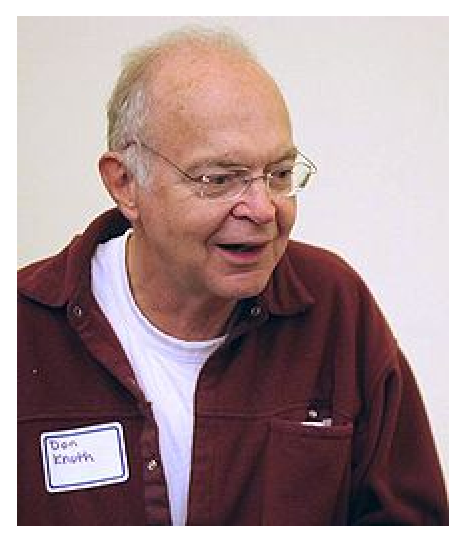
\includegraphics[width=1\linewidth]{knuth1}}
  \end{minipage}
  \hfill
  \begin{minipage}[h]{0.49\linewidth}
    \textbf{Составная \\ подпись 2}
    \center{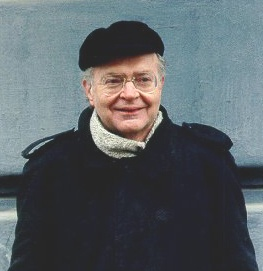
\includegraphics[width=1\linewidth]{knuth2}}
  \end{minipage}
\end{figure}
\end{frame}

\begin{frame}
\frametitle{Таблица}
\begin{tabular}{|l|l|}
\hline
\textbf{Заголовок 1} & \textbf{Заголовок 2} \\
\hline
Сумма & $b+a$ \\
\hline
Разность & $a-b$ \\
\hline
Произведение & $a*b$ \\
\hline
\end{tabular}
\end{frame}

\begin{frame}
\frametitle{Большой многоуровневый список}
\begin{itemize}
  \item \textbf{Пункт 1}
    \begin{itemize}
      \itemi Подпункт 1-1
      \itemi Подпункт 1-2
    \end{itemize}
  \item \textbf{Пункт 2}
    \begin{itemize}
      \itemi Подпункт 2-1
    \end{itemize}
  \item \textbf{Пункт 3}
    \begin{itemize}
      \itemi Подпункт 3-1
      \itemi Подпункт 3-2
    \end{itemize}
  \item \textbf{Пункт 4}
    \begin{itemize}
      \itemi Подпункт 4-1
    \end{itemize}
  \item \textbf{Пункт 5}
    \begin{itemize}
      \itemi Подпункт 5-1
      \itemi Подпункт 5-2
      \itemi Подпункт 5-3
    \end{itemize}
\end{itemize}
\end{frame}

\begin{frame}
\frametitle{Четыре изображения}
\begin{figure}[H]
  \center
    
\includegraphics[width=0.4\linewidth]{latex}
    
\includegraphics[width=0.4\linewidth]{latex}\\
    
\includegraphics[width=0.4\linewidth]{latex}
    
\includegraphics[width=0.4\linewidth]{latex}
\end{figure}
\end{frame}

%%%%%%%%%%%%%%%%%%%%%%%%%%%%%%
\begin{frame}
\frametitle{Перспективы развития проекта}
\begin{itemize}
  \item Перспектива 1
  \item Перспектива 2
  \item Перспектива 3
  \item Перспектива 4
  \item Перспектива 5
\end{itemize}
\end{frame}

\begin{frame}
\frametitle{Результаты работы}
\begin{itemize}
  \item Результат 1
  \item Результат 2
  \item Результат 3
  \item Результат 4
\end{itemize}
\end{frame}

\begin{frame}
\begin{center}
Спасибо за внимание!
\end{center}
\end{frame}

\end{document} 